%%%%%%%%%%%%%%%%%%%%%%%%%%%%%%%%%%%%%%%%%%%%%%%%%%%%%%%%%%%%%

\mainmatter
\setcounter{page}{1}

\lectureseries[\course]{\course}

\auth[\lecAuth]{Lecturer: \lecAuth\\ Scribe: \scribe}
\date{November 17, 2009}

\setaddress

% the following hack starts the lecture numbering at 14
\setcounter{lecture}{13}
\setcounter{chapter}{13}

\lecture{Control with HJB}

\section{Hamilton-Jacobi-Bellman Review}

We set up the system with
\begin{align}
\label{eq:14d}
\dot{\xi} &= f(\xi,u) \\
\label{eq:14ic}
\xi_s &= x\in\mathbb{R}^n
\end{align}
We also have that the Lipschitz condition is satisfied, or
\begin{align}
\label{eq:14l}
\exists ~ K<\infty \text{ s.t. } |f(x,v)-f(y,v)| \leq K|x-y| ~\forall x,y\in\mathbb{R}^n, ~\forall v\in\mathbb{R}^m
\end{align}
Then, let
$$\mathcal{U}_{s,T} = \left\lbrace u:[s,T)\to\mathcal{U} ~|~ ||u||_{L_2(s,T)}<\infty \right\rbrace$$
Also,
\begin{align}
\label{eq:14cset}
\exists ~! \text{ sol to (\ref{eq:14d}) and (\ref{eq:14ic}) } \forall u\in\mathcal{U}_{s,T}
\end{align}
The cost and value functions are given by
\begin{align*}
J(s,x,u) &= \int_s^T l(\xi_t,u_t)dt + \psi(\xi_t) \\
V(s,x) &= \inf_{u\in\mathcal{U}_{s,T}} J(s,x,u)
\end{align*}
The Dynamic Programming Principle (DPP) is
\begin{align}
\label{eq:14dpp}
V(s,x) = \inf_{u\in\mathcal{U}_{s,T}} \left\lbrace \int_s^T l(\xi_t,w_t)dt + V(t,\xi_t) \right\rbrace
\end{align}
Using this, we get the HJB PDE as
\begin{align}
\label{eq:14hjb}
&0 = W_s(s,x) + \inf_{v\in\mathcal{U}} \left\lbrace f(x,v)\cdot\nabla_xW(s,x)+l(x,v) \right\rbrace \\
\label{eq:14tc}
&W(T,x) = \psi(x)
\end{align}
Note that (\ref{eq:14tc}) represent the terminal condition. We saw in Example \ref{ex:13hjb} how to use the HJB PDE. We will make the assumption that
\begin{align}
\label{eq:14ae}
\exists~ !~ C^1 \text{ sol of (\ref{eq:14hjb}), (\ref{eq:14tc}), } W
\end{align}

Let $\uinu_{s,T}$. By (\ref{eq:14cset}) there exists $C^1, \xi_0$ satisfying (\ref{eq:14d}) and (\ref{eq:14ic}). We have that a continuous function on a compact set is bounded which implies
$$\exists~ R=R(s,x,u) \text{ s.t. } |\xi_k|\leq R ~\forall t\in[s,T]$$

Now we want to look at the trajectory of the system under this controller. Consider $W(t,\xi_t)$. We have $W(\cdot,\xi_0)\in C^1[s,T]$ is bounded on the interval $[s,T]$. This lets us use the Fundamental Theorem of Calculus to get
\begin{align*}
W(T,\xi_T) - W(s,\xi_s) &= \int_s^T \frac{d}{dt}[W(t,\xi_t)]dt \\
&= \int_s^T W_s(t,\xi_t) + \nabla_x W(t,\xi_t) \frac{d\xi_t}{dt}dt \\
&= \int_s^TW_s(t,\xi_t) + \nabla_x W(t,\xi_t)\cdot f(\xi_t,u_t)dt
\end{align*}
Looking at (\ref{eq:14dpp}) we see that the infinum term is greater than or equal to zero. So, for any $s,x,u$ we have
\begin{align}
\label{eq:14fxv}
f(x,v)\cdot\nabla_xW(s,x)+W_s \geq -l(x,v)
\end{align}
Substituting (\ref{eq:14fxv}) into (\ref{eq:14dpp}) yields
$$W(T,\xi_T) - W(s,\xi_s) \geq \int_s^T -l(\xi_t,u_t)dt$$
We can re-write this as
$$W(s,\xi_s) \leq \int_s^T l(\xi_t,u_t)dt + W(T,\xi_T)$$
By (\ref{eq:14tc})
$$W(s,x) \leq \int_s^T l(\xi_t,u_t)dt + \psi(\xi_T) = J(s,x,u)$$
This is true $\forall \uinu_s$,
\begin{align}
\label{eq:14wv}
\therefore W(s,x) \leq V(s,x)
\end{align}
More details about this proof can be found in Fleming/Rishel.

Next, suppose there exists $\mu_0(\cdot)$ such that
\begin{align}
\label{eq:14c1d}
\exists~ !~ C^1 \text{ sol of } \dot{\bar{\xi}} = f(\bar{\xi}_t,\bar{\mu}_t(\bar{\xi}_t)), ~\bar{\xi}_s=x
\end{align}
Let $u_t^\ast=\bar{\mu}_t(\bar{\xi}_t)$ and $\dot{\xi}^\ast = f(\xi_t^\ast,\mu_t^\ast)$, $\xi_s^\ast=y$ with $\xi^\ast\equiv\bar{\xi}$. Then
\begin{align}
\label{eq:14fstar}
\begin{split}
&f(\xi_t^\ast,u_t^\ast)\cdot\nabla_xW(t,\xi_t^\ast) + l(\xi_t^\ast,u_t^\ast) = \\
&\qquad \inf_{v\in\mathcal{U}}\left[ f(\xi_t^\ast,v_t)\cdot\nabla_xW(t,\xi_t^\ast) + l(\xi_t^\ast,v) \right] ~\forall t\in[s,T]
\end{split}
\end{align}
Again, by the Fundamental Theorem of Calculus
\begin{align}
\label{eq:14wt}
W(T,\xi_t^\ast)-W(s,x) = \int_s^T f(\xi_t^\ast,u_t^\ast)\cdot\nabla_xW(t,\xi_t^\ast)+W_s(t,\xi_t^\ast)dt
\end{align}
By (\ref{eq:14fstar}) and (\ref{eq:14hjb})
\begin{align}
\label{eq:14ws}
W_s(t,\xi_t^\ast) + f(s^\ast,u^\ast)\cdot\nabla_xW(t,\xi_t^\ast) + l(\xi_t^\ast,u_t^\ast) = 0
\end{align}
Substituting (\ref{eq:14ws}) into (\ref{eq:14wt})
\begin{align}
\label{eq:14wsx}
W(T,\xi_t^\ast) - W(s,x) &= \int_s^T -l(\xi_t^\ast,u_t^\ast)dt \nonumber \\
W(s,x) = J(s,x,u^\ast) &\geq V(s,x)
\end{align}

\begin{theorem}
Suppose (\ref{eq:14l}) and (\ref{eq:14ae}) and let $W$ be the solution of (\ref{eq:14hjb}) and (\ref{eq:14ic}), then $W\subseteq V$. Further, if there exists $\bar{\mu}$ satisfying (\ref{eq:14c1d}) and (\ref{eq:14fstar}) then
$$W=V=J(s,x,u^\ast)$$
with $u_t^\ast = \bar{\mu}_t(\bar{\xi}_t)$.
\end{theorem}

\textit{Exercise}: Suppose there exists an $\epsilon$-optimal $\bar{\mu}^\epsilon$ satisfying (\ref{eq:14c1d}) and
\begin{align}
\label{eq:14feps}
f(\xi^\epsilon,u_t^\epsilon)\cdot\nabla_xW(t,\xi_t^\epsilon) + l(\xi_t^\epsilon,u_t^\epsilon) \leq \inf_{v\in\mathcal{U}} \left\lbrace f(\xi^\epsilon,v)\cdot\nabla_x W(t,\xi_t^\epsilon) + l(\xi_t^\epsilon,v) \right\rbrace + \epsilon
\end{align}
with $u_t^\epsilon\doteq \bar{\mu}_t^\epsilon(\xi_t^\epsilon)$ and $\dot{\xi}_t^\epsilon = f(\xi_t^\epsilon, \bar{\mu}_t^\epsilon(\xi_t^\epsilon))$. Then $W\geq V$. Further, $J(s,x,u^\epsilon) \leq V(s,x) + \epsilon(T-s)$. Prove this as an exercise.

\begin{example}
\label{ex:14lq}
The LQ control problem is set up as
\begin{align*}
&\dot{\xi} = A\xi_t+Bu_t \\
&\xi_s = x_0 \\
&J(s,x,u) = \int_s^T\tfrac{1}{2}\xi_t^TC\xi_t + \tfrac{1}{2}u_t^TDu_tdt + \tfrac{1}{2}(\xi_T-z)^TE(\xi_T-z) \\
&0 = W_{s,T} + \min\left\lbrace (Ax)^T\nabla_xW + (Bv)^T\nabla_xW + \tfrac{1}{2}x^TCx + \tfrac{1}{2}v^TDv \right\rbrace \\
&v^TB^T\nabla_xW + \frac{1}{2}v^TDV = 0 \\
&B^T\nabla_xW + Dv = 0
\end{align*}
The terminal condition is given by
\begin{align}
\label{eq:14extc}
W(T,x) &= \tfrac{1}{2}(x-z)^TE(x-z)
\end{align}
Let $D^{-1}$ exist, then
\begin{align*}
v^\sigma &= -D^{-1}B^T\nabla_xW \\
0 &= W_x+\underbrace{x^TA^T\nabla_xW}_{\lambda} + \tfrac{1}{2}x^TCx - \tfrac{1}{2}\nabla_xW^T\Sigma\nabla_xW
\end{align*}
where $\Sigma = -BD^{-1}B^T$.

Suppose
$$W(t,x) = \tfrac{1}{2}(x-\bar{x}_t)^TP_t(x-\bar{x}_t) + r_t$$
From (\ref{eq:14extc}) $\bar{x}_T = z$, $P_T=E$ and $r_T=0$. Then
\begin{align*}
W_t &= \tfrac{1}{2}(x-\bar{x}_t)^T\dot{P}_t(x-\bar{x}_t)+\dot{r}_t - \tfrac{1}{2}\dot{\bar{x}}^TP_t(x-\bar{x}_t) - \tfrac{1}{2}(x-\bar{x}_t)^TP_t\dot{\bar{x}}_t \\
\nabla_xW &= P_t(x-\bar{x}_t) \\
0 &= \tfrac{1}{2}(x-\bar{x}_t)^T\dot{P}_t(x-\bar{x}_t) + \dot{r}_t - \tfrac{1}{2}\dot{\bar{x}}_tP_t(x-\bar{x}_t) - \tfrac{1}{2}(x-\bar{x}_t)^TP_t\dot{\bar{x}}_t \\
&\qquad + \underbrace{\tfrac{1}{2}x^TAP_t(x-\bar{x}_t) + \tfrac{1}{2}(x-\bar{x}_t)^TP_tA^Tx}_{\lambda} + \tfrac{1}{2}x^TCx \\
&\qquad - \tfrac{1}{2}(x-\bar{x}_t)^TP_t\Sigma P_t(x-\bar{x}_t)
\end{align*}
Notice that $\lambda$ is a scalar value and $P_t$ is symmetric so the term $x^TA^T\nabla_xW$ was separated into two components above.

Since we are using a quadratic form for the cost function it is of the form $a(t)x^2+b(t)x+c(t)$ and we want this to be equal to zero for all $t$ and $x$. The only way for that to occur is if $a(t)=b(t)=c(t)=0$. Looking at the quadratic terms such that $a(t)=0$ gives the Riccati equation as
\begin{align*}
0 &= \tfrac{1}{2}\dot{P}_t + \tfrac{1}{2}AP_t + \tfrac{1}{2}P_tA^T + \tfrac{1}{2}C - \tfrac{1}{2}P_t\Sigma P_t \\
\Rightarrow \dot{P}_t &= -AP_t - P_tA^T - C + P_t\Sigma P_t
\end{align*}
Next, we separate out the $x^T(\cdot)$ and $(\cdot)x$ linear terms and find $b(t) = 0$ such that
\begin{align*}
0 &= -\tfrac{1}{2}\dot{P}_t\bar{x}_t - \tfrac{1}{2}P_t\dot{\bar{x}}_t - \tfrac{1}{2}AP_t\bar{x}_t + \tfrac{1}{2}P_t\Sigma P_t\bar{x}_t \\
P_t\dot{\bar{x}}_t &= -\dot{P}_t\bar{x}_t - AP_t\bar{x}_t + P_t\Sigma P_t\bar{x}_t \\
\dot{\bar{x}}_t &= P_t^{-1}\left[ (AP_t+P_tA^T+C-P_t\Sigma P_t)\bar{x}_t - AP_t\bar{x}_t + P_t\Sigma P_t\bar{x}_t \right] \\
&= P_t^{-1}\left[P_tA^T + C\right] \bar{x}_t
\end{align*}
$\lozenge$
\end{example}

\section{Exit Problem}
This is for deterministic control. The system is given as
$$\dot{\xi} = f(\xi,u), \qquad \xi_0 = x\in G$$
Here, $G$ is an open set and $\bar{G}$ is a compact set. Recall that $G$ is open if and only if given
$$x\in G, ~\exists~ \delta_x \text{ s.t. } B_{\delta_x}(x)\subset G$$
Let
$$\partial G = \{x\in\mathbb{R}^n ~|~ x\notin G, x\notin(G^C)^0\}$$
be the boundary of $G$. Let
$$\tau = \inf\{t\geq 0 ~|~ \xi_t\notin G\}$$
Note that $\tau=\tau(x,u)$. Let
$$\mathcal{U}_0 = \{u:[0,\infty)\to\mathcal{U} ~|~ ||u||_{L_2[0,T]}<\infty ~\forall T\}$$
Let
$$\mathcal{U}_0^\ast = \{\uinu_0 ~|~ \tau=\tau(x,u)<\infty\}$$
This means that the system is controllable. We will assume $\mathcal{U}_0^\ast\neq\emptyset ~\forall x\in G$. The cost function is then
$$J(x,u) = \int_u^\tau l(\xi_t,u_t)dt + \psi(\xi_\tau)$$
where $\psi(\xi_\tau)$ is the exit cost. Now we get the HJB PDE as
\begin{align}
\label{eq:14ephjb}
0 = \inf_{v\in\mathcal{U}} \left\lbrace f(x,v)\cdot\nabla_xW(x) + l(x,u) \right\rbrace
\end{align}
for $x\in G$. The boundary condition is
\begin{align}
\label{eq:14epbc}
W(x) = \psi(x), \qquad x\in\partial G
\end{align}
The argument goes that we assume there exists a unique $C^1$ solution of (\ref{eq:14ephjb}) and (\ref{eq:14epbc}). Then we use the Fundamental Theorem of Calculus to get
$$W(\xi_\tau) - W(\xi_0) = \int_0^\tau \nabla_xW(\xi_t)f(\xi_t,u_t)dt$$
As before in computing (\ref{eq:14fxv}) we know that one part of the infinum is greater than or equal to zero which implies
\begin{align*}
\psi(\xi_t) - W(x) &\geq \int_0^\tau -l(\xi_t,u_t)dt \\
W(x) &\leq \int_0^\tau l(\xi_t,u_t)dt + \psi(\xi_t)
\end{align*}
This is true $\forall \uinu_0^\ast$
$$\therefore W(x)\leq V(x) ~\forall x$$
It is the same idea as for optimal control.

\begin{example}
\label{ex:14exit}
Let the system be described by
\begin{align*}
\dot{\xi} = A\xi+Bu, \qquad \xi_0 = x, \qquad G=B_R(0)
\end{align*}
We are looking at a space that is a ball with radius $R$ around the origin, see Figure \ref{fig:14circle}. The cost function is
$$J(x,u) = \int_0^\tau \rho + \tfrac{1}{2}|u_t|^2dt, \qquad \rho>0$$
Now we go to the HJB PDE and find
\begin{align*}
&W(x) = 0, \qquad |x|=R \\
&0 = \min_{u\in\mathbb{R}^m} \left\lbrace x^TA^T\nabla_xW + u^TB^T\nabla_xu + \rho + \tfrac{1}{2}|u_t|^2 \right\rbrace \\
&0 = \rho + x^TA^T\nabla_xW - \tfrac{1}{2}\nabla_xWBB^T\nabla_xW
\end{align*}
Suppose $A=0$ and $B=I$, then
\begin{align}
\label{eq:14exrho}
&0 = \rho - \tfrac{1}{2}|\nabla_xW|^2 \nonumber \\
\Rightarrow &|\nabla_xW| = \sqrt{2\rho}
\end{align}
We guess that
$$\nabla_xW(x) = \pm \sqrt{2\rho}\frac{x}{|x|}$$
satisfies (\ref{eq:14exrho}). This leads to
$$\Rightarrow W(x) = \pm\sqrt{2\rho}|x|+C = \pm\sqrt{2\rho}(|x|-R)$$
Since $\rho>0$ we get
$$W(x) = \sqrt{2\rho}(R-|x|)$$
Notice that this is not differentiable at $x=0$. This property is not unique to this example but is found in general for these types of problems.
$\lozenge$
\end{example}

\begin{figure}[ht!]
	\centering
	\includegraphics[width=.4\textwidth]{images/14circle}
	\caption{Space that is a ball with radius $R$ around the origin.}
	\label{fig:14circle}
\end{figure}

%%%%%%%%%%%%%%%%%%%%%%%%%%%%%%%%%%%%%%%%%%%%%%%%%%%%%%%%%%%%%